\documentclass[11pt]{article}
\usepackage{amsfonts,amsthm,amsmath,amssymb, hyperref, dsfont, enumitem, bbm}
\usepackage{array}
\usepackage{epsfig}
\usepackage{fullpage}
\usepackage{color}
\usepackage{epigraph}
\renewcommand{\epigraphflush}{center}
\usepackage[framemethod=tikz]{mdframed}
\usepackage{titlesec}
\usepackage{ellipsis}
\usepackage{subcaption}
\usepackage[normalem]{ulem}
\usepackage{todonotes}



\titleformat{\chapter}[display]
  {\normalfont\bfseries}{}{0pt}{\Huge}

\newif\ifdetails % fill in details that are omitted in lecture handout version


\newcommand{\qn}[1]{\todo[inline, color=brown!30]{Quynh: #1}}

% \newtheorem{theorem}{Theorem}[section]
% \newtheorem{definition}[theorem]{Definition}
% \newtheorem{lemma}[theorem]{Lemma}
% \newtheorem{corollary}[theorem]{Corollary}
% \newtheorem{proposition}[theorem]{Proposition}
% \newtheorem{example}[theorem]{Example}
% \newtheorem{remark}[theorem]{Remark}

\newcommand{\R}{\mathbb{R}} 
\newcommand{\x}{\mathbf{x}} 
\newcommand{\y}{\mathbf{y}} 
\newcommand{\bb}{\mathbf{b}} 
\newcommand{\id}{\mathbbm{1}} 


\detailstrue %Change to detailsfalse when removing text

\begin{document}

%% Courtesy: Daniel Spielman, via Madhu Sudan --> Chi-Ning Chou --> Anurag Anshu

\theoremstyle{plain}
\newtheorem{theorem}{Theorem}[section]
\newtheorem{lemma}[theorem]{Lemma}
\newtheorem{example}[theorem]{Example}
\newtheorem{corollary}[theorem]{Corollary}
\theoremstyle{definition}
\newtheorem{definition}[theorem]{Definition}
\newtheorem*{mydefinition}{Definition}
\newtheorem{claim}[theorem]{Claim}
\newtheorem{fact}[theorem]{Fact}
\newtheorem{remark}[theorem]{Remark}
\newtheorem{exercise}[theorem]{Exercise}

%Left and right brackets
\newcommand {\br} [1] {\ensuremath{ \left( #1 \right) }}
\newcommand {\Br} [1] {\ensuremath{ \left[ #1 \right] }}


%Quantum notations
\newcommand {\norm}[1]{{\| #1 \|}}  
\newcommand {\bra} [1] {\ensuremath{ \left\langle #1 \right| }}
\newcommand {\ket} [1] {\ensuremath{ \left| #1 \right\rangle }}
\newcommand {\ketbratwo} [2] {\ensuremath{ \left| #1 \middle\rangle \middle\langle #2 \right| }}
\newcommand {\ketbra} [1] {\ketbratwo{#1}{#1}}
\newcommand{\braket}[2]{\langle#1|#2\rangle}
\newcommand{\Tr}[1]{\mathrm{Tr}\left(#1\right)}
\newcommand{\tr}[2]{\mathrm{Tr}_{#1}\left(#2\right)}
\newcommand{\PE}{\mathrm{PE}}
\newcommand{\EPR}{\mathrm{EPR}}
\newcommand{\CNOT}{\mathrm{CNOT}}
\newcommand{\CZ}{\mathrm{CZ}}

%Generic math symbols
\newcommand {\eps} {\varepsilon}
\newcommand{\tO}{\tilde{O}}
\newcommand{\ind}[1]{\mathrm{Ind}\left(#1\right)}
\newcommand {\id}{\mathds{1}}
\newcommand{\bitn}[1]{\ensuremath{\{0,1\}^{#1}}}
\newcommand{\bitone}{\ensuremath{\{0,1\}}}
\newcommand{\swp}{\mathrm{\textbf{Swap}}}

% Information theory and CS symbols
\newcommand {\prob} {\ensuremath{\mathrm{Prob}}}
\newcommand{\bigo}[1]{\mathcal{O}\left(#1\right)}
\newcommand{\omeg}[1]{\Omega\left(#1\right)}
\newcommand{\expec}{\mathbb{E}}
\newcommand{\relent}[2]{\mathrm{D}\left(#1\|#2\right)}
\newcommand{\KL}[2]{\mathrm{D}_{KL}\left(#1\|#2\right)}
\newcommand{\mutinf}[2]{\mathrm{I}\left(#1:#2\right)}
\newcommand{\condmutinf}[3]{\mathrm{I}\left(#1:#2|#3\right)}
\newcommand{\condent}[2]{\mathrm{S}\left(#1|#2\right)}
\newcommand{\ent}[1]{\mathrm{S}\left(#1\right)}
\newcommand{\cla}{\text{classical}}
\newcommand{\qua}{\text{quantum}}
\newcommand{\sym}{\textsf{sym}}

%Statistical measures
\newcommand{\F}{\mathrm{F}}
\newcommand{\tv}{\mathrm{TV}}
\newcommand{\Hol}{\mathrm{Hol}}
\newcommand{\hel}{\mathrm{Hd}}
\newcommand{\pur}{\mathrm{Pur}}
\newcommand{\scs}{\mathrm{succ}}
\newcommand{\err}{\mathrm{err}}
\newcommand{\can}{\mathrm{can}}
\newcommand{\Var}{\mathrm{Var}}

%Fancy alphabets
\def\cA{\mathcal{A}}
\def\cB{\mathcal{B}}
\def\cC{\mathcal{C}}
\def\cD{\mathcal{D}}
\def\cE{\mathcal{E}}
\def\cF{\mathcal{F}}
\def\cG{\mathcal{G}}
\def\cH{\mathcal{H}}
\def\cL{\mathcal{L}}
\def\cM{\mathcal{M}}
\def\cO{\mathcal{O}}
\def\cP{\mathcal{P}}
\def\cR{\mathcal{R}}
\def\cS{\mathcal{S}}
\def\cT{\mathcal{T}}
\def\cX{\mathcal{X}}
\def\N{\mathbb{N}}
\def\Z{\mathbb{Z}}



%%%%%%%%%%%%%%%%%%%%%%%%%%%%%%%%%%%%%%%%%%%%% 
%Commands below can be ignored by the students  
%%%%%%%%%%%%%%%%%%%%%%%%%%%%%%%%%%%%%%%%%%%%%
% Header
\newcommand{\handout}[5]{
   \renewcommand{\thepage}{#1-\arabic{page}}
   \noindent
   \begin{center}
   \framebox{
      \vbox{
    \hbox to 6.3in { {\bf #1}
     	 \hfill {\it #3} }
       \vspace{4mm}
       \hbox to 6.3in { {\Large \hfill #5  \hfill} }
       \vspace{2mm}
       \hbox to 6.3in { {\it #2 \hfill #4} }
      }
   }
   \end{center}
   \vspace*{4mm}
}

\newcommand{\lecture}[4]{\handout{#1}{#2}{Lecturer:
#3}{Scribe: #4}{Lecture #1}}



%Editing commands
\newcommand{\edit}[2]{\st{#1}\hspace{0.05in}\textcolor{blue}{#2}}
\newcommand{\suppress}[1]{}

\newcommand{\anote}[1]{{\color{red} \textbf{Anurag's note:} #1}}
\newcommand{\qnote}[1]{{\color{red} \textbf{Quynh's note:} #1}}
\newcommand{\hkn}[1]{{\color{orange} \textbf{Nguyen nu:} #1}}


%Itemizing and Equation shorthands
\newcommand{\beit}{\begin{itemize}}
\newcommand{\enit}{\end{itemize}}
\newcommand{\been}{\begin{enumerate}}
\newcommand{\enen}{\end{enumerate}}
\newcommand{\beq}{\begin{equation}}
\newcommand{\enq}{\end{equation}}
\newcommand{\beqst}{\begin{equation*}}
\newcommand{\enqst}{\end{equation*}}
\newcommand{\beqar}{\begin{eqnarray}}
\newcommand{\enqar}{\end{eqnarray}}
\newcommand{\beqarst}{\begin{eqnarray*}}
\newcommand{\enqarst}{\end{eqnarray*}}




\handout{SEAS 2025}{{\bf July ..., 2025}}{Instructor: }{TA: }{Lecture 3: Eigendecomposition and Spectral theorem}

In charge: Nguyen nam

\section{Solving Lots of Equations at Once}

Recall that a fundamental problem in linear algebra is solving a system of linear equations. Such a system, consisting of $m$ equations in $n$ unknowns, can be compactly represented in matrix form:
\begin{align*}
    2x + 3y &= 7 \\
    x - y &= 1
\end{align*}
We can solve these using substitution or elimination. But what if we have 10 equations and 10 unknowns? Or 100? We need a more organized way. Linear algebra gives us that using matrices.

We can write the system above as a matrix equation:
\[ \underbrace{\begin{bmatrix} 2 & 3 \\ 1 & -1 \end{bmatrix}}_{A} \underbrace{\begin{bmatrix} x \\ y \end{bmatrix}}_{\x} = \underbrace{\begin{bmatrix} 7 \\ 1 \end{bmatrix}}_{\bb} \]
This is in the form $A\x = \bb$, where $A$ is the matrix of coefficients, $\x$ is the vector of variables we want to find, and $\bb$ is the vector of constants on the right side. Our goal is to find $\x$.

\section{The Matrix Inverse: Undoing a Matrix}

Think about a simple equation like $5x = 10$. To solve for $x$, you multiply by the reciprocal (or inverse) of 5, which is $1/5$: $(1/5) \times 5x = (1/5) \times 10$, so $1x = 2$, or $x=2$. We want something similar for matrices.

\subsection{The Identity Matrix: The Matrix Version of '1'}

First, we need a matrix that acts like the number 1. This is the \textbf{identity matrix}, $\id$. It's a square matrix with 1s on the main diagonal (top-left to bottom-right) and 0s everywhere else.
\[ \id_2 = \begin{bmatrix} 1 & 0 \\ 0 & 1 \end{bmatrix} \quad \text{(2x2 identity)}, \qquad \id_3 = \begin{bmatrix} 1 & 0 & 0 \\ 0 & 1 & 0 \\ 0 & 0 & 1 \end{bmatrix} \quad \text{(3x3 identity)} \]
Just like $1 \times x = x$, multiplying by $\id$ doesn't change a vector or matrix:
\[ A \id = A, \quad \id A = A, \quad \id \x = \x \]

\subsection{The Inverse Matrix:  The Matrix Version of '1/5'}

For \textit{some} square matrices $A$, there's a special matrix called the \textbf{inverse matrix}, written $A^{-1}$ (read "A inverse"). It's the matrix that "undoes" $A$. When you multiply $A$ by its inverse $A^{-1}$ (in either order), you get the identity matrix $\id$:
\[ A A^{-1} = \id \quad \text{and} \quad A^{-1} A = \id \]

\begin{remark}
\begin{itemize}
    \item Only square matrices ($n \times n$) might have an inverse.
    \item Not all square matrices have an inverse! If a matrix \textit{does} have an inverse, it's called \textbf{invertible}. If it doesn't, it's called \textbf{singular}.
    \item If an inverse exists, it's unique for that matrix $A$.
\end{itemize}
\end{remark}

\subsection{Using the Inverse to Solve Equations}

If our matrix $A$ in the equation $A\x = \bb$ is invertible, we can solve for $\x$ just like the simple $5x=10$ example. Multiply both sides (on the left!) by $A^{-1}$:
\begin{align*}
    A\x &= \bb \\
    A^{-1} (A\x) &= A^{-1} \bb && \text{(Multiply both sides on the left by } A^{-1} \text{)} \\
    (A^{-1} A) \x &= A^{-1} \bb && \text{(Group matrices)} \\
    \id \x &= A^{-1} \bb && \text{(Since } A^{-1}A = \id \text{)} \\
    \x &= A^{-1} \bb && \text{(Since } \id\x = \x \text{)}
\end{align*}
So, if we know $A^{-1}$, we have a direct formula to find the solution: $\x = A^{-1}\bb$. This formula only works if $A$ is square and invertible. An invertible matrix $A$ guarantees that the system $A\x=\bb$ has exactly one unique solution for any $\bb$.

This is great, but two questions remain:
\begin{enumerate}
    \item How can we tell if $A^{-1}$ exists without trying to find it? (We'll see later that the determinant helps here!)\
    \item If $A^{-1}$ does exist, how do we actually calculate it (or solve the system directly)?
\end{enumerate}

The answer to the second question is a method called \textbf{Gauss-Jordan Elimination}.

\section{Gauss-Jordan Elimination: The Systematic Solving Method}

Gauss-Jordan Elimination is a step-by-step process using simple row manipulations to solve $A\x = \bb$ or to find $A^{-1}$. It's like the elimination method you learned for small systems, but super organized.

\subsection{The Augmented Matrix: Keeping Track}

To start, we combine $A$ and $\bb$ into a single "augmented" matrix. We just write the columns of $A$ and then add the column $\bb$, often separated by a vertical line for clarity.
For our example system $\begin{bmatrix} 2 & 3 \\ 1 & -1 \end{bmatrix} \begin{bmatrix} x \\ y \end{bmatrix} = \begin{bmatrix} 7 \\ 1 \end{bmatrix}$, the augmented matrix is:
\[ [A \mid \bb] = \left[ \begin{array}{cc|c} 2 & 3 & 7 \\ 1 & -1 & 1 \end{array} \right] \]
Now, we'll apply some "legal moves" to the rows of this augmented matrix.

\subsection{Elementary Row Operations (EROs): The Legal Moves}

These are the three operations we're allowed to do on the rows of the augmented matrix. They change how the matrix looks but \textit{don't change the solution} of the original system.
\begin{enumerate}
    \item \textbf{Row Swapping:} Interchange row $i$ and row $j$. Notation: $R_i \leftrightarrow R_j$.
    \[ \left[\begin{array}{c} \vdots \\ \text{row}_i(A) \\ \vdots \\ \text{row}_j(A) \\ \vdots \end{array}\right] \xrightarrow{R_i \leftrightarrow R_j} \left[\begin{array}{c} \vdots \\ \text{row}_j(A) \\ \vdots \\ \text{row}_i(A) \\ \vdots \end{array}\right] \]
    \item \textbf{Scalar Multiplication:} Multiply row $i$ by a non-zero scalar $c$. Notation: $c R_i \to R_i$.
    \[ \left[\begin{array}{c} \vdots \\ \text{row}_i(A) \\ \vdots \end{array}\right] \xrightarrow{c R_i \to R_i} \left[\begin{array}{c} \vdots \\ c \cdot \text{row}_i(A) \\ \vdots \end{array}\right] \quad (c \neq 0) \]
    \item \textbf{Row Addition:} Add a multiple ($c$) of row $j$ to row $i$. Notation: $R_i + c R_j \to R_i$.
    \[ \left[\begin{array}{c} \vdots \\ \text{row}_i(A) \\ \vdots \\ \text{row}_j(A) \\ \vdots \end{array}\right] \xrightarrow{R_i + c R_j \to R_i} \left[\begin{array}{c} \vdots \\ \text{row}_i(A)+c \cdot \text{row}_j(A) \\ \vdots \\ \text{row}_j(A) \\ \vdots \end{array}\right] \]
\end{enumerate}

These are basically the steps you use in regular elimination (swapping equations, multiplying an equation by a number, adding one equation to another).

\subsection{The Goal: Reaching the Solution}

Our aim is to use these EROs to turn the left side (the $A$ part) of the augmented matrix into the identity matrix $\id$. If we can do that, the right side will automatically become the solution vector $\x$ (because $\id \x = \x$).
\[ [A \mid \bb] \xrightarrow{\text{Apply EROs}} [\id \mid \x] \]

Let's solve our example system $\left[ \begin{array}{cc|c} 2 & 3 & 7 \\ 1 & -1 & 1 \end{array} \right]$:

\begin{example}[Solving $A\x=\bb$]
\begin{align*}
\left[ \begin{array}{cc|c} 2 & 3 & 7 \\ 1 & -1 & 1 \end{array} \right]
&\xrightarrow{R_1 \leftrightarrow R_2} && \text{Swap rows to get a 1 in the top-left} \\
\left[ \begin{array}{cc|c} 1 & -1 & 1 \\ 2 & 3 & 7 \end{array} \right]
&\xrightarrow{R_2 - 2R_1 \to R_2} && \text{Make the 2 below the leading 1 into a 0} \\
\left[ \begin{array}{cc|c} 1 & -1 & 1 \\ 0 & 5 & 5 \end{array} \right]
&\xrightarrow{\frac{1}{5} R_2 \to R_2} && \text{Make the leading entry in R2 into a 1} \\
\left[ \begin{array}{cc|c} 1 & -1 & 1 \\ 0 & 1 & 1 \end{array} \right]
&\xrightarrow{R_1 + R_2 \to R_1} && \text{Make the -1 above the leading 1 in R2 into a 0} \\
\left[ \begin{array}{cc|c} 1 & 0 & 2 \\ 0 & 1 & 1 \end{array} \right]
\end{align*}
Now the left side is $\id_2$. The right side gives the solution! $\begin{bmatrix} x \\ y \end{bmatrix} = \begin{bmatrix} 2 \\ 1 \end{bmatrix}$, so $x=2$ and $y=1$.
\end{example}

\begin{remark}
Sometimes, you might get a row like $[0 \ 0 \mid 5]$ during the process. This means $0x + 0y = 5$, which is impossible! So the system has \textbf{no solution}. If you get a row like $[0 \ 0 \mid 0]$, it means $0x+0y=0$, which is always true and usually indicates \textbf{infinitely many solutions} (if you have fewer non-zero rows than variables). This happens when the original matrix $A$ was singular (not invertible).
\end{remark}

\subsection{Using Gauss-Jordan to Find the Inverse}

We can use the exact same process to find $A^{-1}$. Instead of augmenting $A$ with $\bb$, we augment it with the identity matrix $\id$. Then we apply EROs to turn the left side ($A$) into $\id$. The right side, which started as $\id$, will magically turn into $A^{-1}$.
\[ [A \mid \id] \xrightarrow{\text{Apply EROs}} [\id \mid A^{-1}] \]

Why does this work? The sequence of EROs that transforms $A$ into $\id$ is like multiplying $A$ by $A^{-1}$. If we apply the exact same sequence of operations to $\id$, we are effectively calculating $A^{-1} \id$, which is just $A^{-1}$.

\begin{example}[Finding $A^{-1}$]
Let's find the inverse of $A = \begin{bmatrix} 2 & 3 \\ 1 & -1 \end{bmatrix}$. We start with $[A \mid \id]$:
\[ \left[ \begin{array}{cc|cc} 2 & 3 & 1 & 0 \\ 1 & -1 & 0 & 1 \end{array} \right] \]
Apply the same EROs as in the previous example:
\begin{align*}
&\xrightarrow{R_1 \leftrightarrow R_2}
\left[ \begin{array}{cc|cc} 1 & -1 & 0 & 1 \\ 2 & 3 & 1 & 0 \end{array} \right] \\
&\xrightarrow{R_2 - 2R_1 \to R_2}
\left[ \begin{array}{cc|cc} 1 & -1 & 0 & 1 \\ 0 & 5 & 1 & -2 \end{array} \right] \\
&\xrightarrow{\frac{1}{5} R_2 \to R_2}
\left[ \begin{array}{cc|cc} 1 & -1 & 0 & 1 \\ 0 & 1 & 1/5 & -2/5 \end{array} \right] \\
&\xrightarrow{R_1 + R_2 \to R_1}
\left[ \begin{array}{cc|cc} 1 & 0 & 1/5 & 3/5 \\ 0 & 1 & 1/5 & -2/5 \end{array} \right]
\end{align*}
The left side is now $\id$. The right side must be $A^{-1}$.
\[ A^{-1} = \begin{bmatrix} 1/5 & 3/5 \\ 1/5 & -2/5 \end{bmatrix} \]
You can check that $A A^{-1} = \id$! Now we could use this inverse to solve $A\x = \begin{bmatrix} 7 \\ 1 \end{bmatrix}$:
\[ \x = A^{-1}\bb = \begin{bmatrix} 1/5 & 3/5 \\ 1/5 & -2/5 \end{bmatrix} \begin{bmatrix} 7 \\ 1 \end{bmatrix} = \begin{bmatrix} (1/5)(7) + (3/5)(1) \\ (1/5)(7) + (-2/5)(1) \end{bmatrix} = \begin{bmatrix} 10/5 \\ 5/5 \end{bmatrix} = \begin{bmatrix} 2 \\ 1 \end{bmatrix} \]
Which matches the solution we found earlier.
\end{example}

So, Gauss-Jordan elimination is our fundamental tool for both solving systems directly ($[A \mid \bb] \to [\id \mid \x]$) and finding the inverse matrix ($[A \mid \id] \to [\id \mid A^{-1}]$), which then allows us to use the formula $\x = A^{-1}\bb$.


\section{The Determinant: A Special Number from a Square Matrix}

We saw earlier that some square matrices $A$ have an inverse $A^{-1}$, and some don't (they are called singular). It would be really useful to have a quick way to tell if a matrix is invertible without having to go through the whole Gauss-Jordan process. That's where the \textbf{determinant} comes in!

The determinant is a single number calculated from a \textit{square} matrix. We write it as $\det(A)$ or sometimes using vertical bars like $|A|$.

\subsection{What does the determinant tell us?}

The most important property for us right now is:

\begin{center}
\textit{A square matrix $A$ is invertible if and only if its determinant is non-zero.} \\
($A^{-1}$ exists $\iff \det(A) \neq 0$)
\end{center}

So, if we calculate this number and it's not zero, we know the matrix has an inverse, the system $A\x = \bb$ has a unique solution for any $\bb$, and the columns of $A$ are linearly independent. If the determinant is zero, the matrix is singular (not invertible).

\subsection{Calculating the Determinant}

\subsubsection{For a 2x2 Matrix}
This is the simplest case. For a matrix $A = \begin{bmatrix} a & b \\ c & d \end{bmatrix}$, the determinant is:
\[ \det(A) = \left| \begin{matrix} a & b \\ c & d \end{matrix} \right| = ad - bc \]
It's the product of the main diagonal elements minus the product of the off-diagonal elements.

\begin{example}
Let $A = \begin{bmatrix} 2 & 4 \\ 1 & 3 \end{bmatrix}$. We found its inverse earlier. Let's check its determinant:
\[ \det(A) = (2)(3) - (4)(1) = 6 - 4 = 2 \]
Since $\det(A) = 2 \neq 0$, the matrix is invertible, which we already knew!

Let $B = \begin{bmatrix} 1 & 2 \\ 2 & 4 \end{bmatrix}$.
\[ \det(B) = (1)(4) - (2)(2) = 4 - 4 = 0 \]
Since $\det(B) = 0$, this matrix $B$ is singular (it does not have an inverse). Try running Gauss-Jordan elimination on $[B \mid I]$ and see what happens! You'll find you get a row of zeros on the left side.
\end{example}

\subsubsection{For a 3x3 Matrix (Optional: Rule of Sarrus)}
For $A = \begin{bmatrix} a & b & c \\ d & e & f \\ g & h & i \end{bmatrix}$, there's a diagonal rule (Rule of Sarrus):
\[ \det(A) = aei + bfg + cdh - ceg - bdi - afh \]
You can visualize this by copying the first two columns to the right of the matrix and taking products along the diagonals:
\[
\left| \begin{matrix} a & b & c \\ d & e & f \\ g & h & i \end{matrix} \right|
\begin{matrix} a & b \\ d & e \\ g & h \end{matrix}
\quad \longrightarrow \quad
\begin{array}{c} \text{Sum of products of} \\ \text{downward diagonals} \\ (aei + bfg + cdh) \end{array}
-
\begin{array}{c} \text{Sum of products of} \\ \text{upward diagonals} \\ (ceg + afh + bdi) \end{array}
\]
\textit{Warning:} This diagonal trick ONLY works for 3x3 matrices! For larger matrices, other methods like cofactor expansion are needed, but we won't detail them here. The key takeaway is that the determinant is a specific number calculated from the matrix entries.

\subsection{Geometric Meaning}
For a $2 \times 2$ matrix $A = [\mathbf{v}_1 \mid \mathbf{v}_2]$, where $\mathbf{v}_1, \mathbf{v}_2$ are the column vectors, $|\det(A)|$ represents the \textbf{area} of the parallelogram formed by $\mathbf{v}_1$ and $\mathbf{v}_2$.
For a $3 \times 3$ matrix, $|\det(A)|$ represents the \textbf{volume} of the parallelepiped (a slanted box) formed by its three column vectors.

\begin{figure}[h]
    \centering
    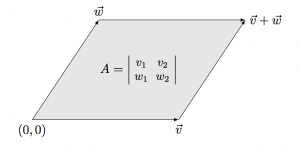
\includegraphics[width=0.4\linewidth]{LA Lecture notes/figures/lec3_det.png}
    \caption{Caption}
\end{figure}

If the determinant is zero, it means the vectors are linearly dependent (e.g., for 2x2, they lie on the same line; for 3x3, they lie on the same plane). This results in a "flat" parallelogram (zero area) or a "flat" box (zero volume), corresponding to the matrix being singular.












\end{document}